%\documentclass{acm_proc_article-sp}
\documentclass{achemso}
\usepackage[latin1]{inputenc}
\usepackage{amsmath}
\usepackage{amsfonts}
\usepackage{multirow}
\usepackage{subcaption}
\usepackage{amssymb}
\usepackage{graphicx}
\title{Validating Complex Interval-Based Temporal Queries over Streams}
%\numberofauthors{1}
\author{
%\alignauthor
Philip Dasler and Sana Malik}
%\affaddr{Department of Computer Science}\\
%\affaddr{University of Maryland}\\
%\affaddr{College Park, MD 20740}\\
\affiliation{University of Maryland, College Park, MD 20740}
\email{{daslerpc, maliks}@cs.umd.edu}

\begin{document}
\maketitle
\begin{abstract}
%Abstract here.
Streaming databases have been growing in popularity as the availability of large datasets gathered in real-time has steadily increased.  Along with the ability to gather and store this data, one must also consider the various concerns involved in processing this data.  More specifically, the performance of queries over such databases is highly dependent on the complexity of the query and the database itself.  These considerations are common in analyses of database systems.  However, on 
\end{abstract}
\section{Introduction}
The ability to query a database for temporal events has become increasingly important as the availability of streaming data has skyrocketed across multiple domains. While event stream processing has seen much work~\cite{Agrawal:2008, Akdere:2008, Ding:2008, Wu:2006, Brenna:2007, Li:2009, Li:2010, Liu:2009}, it has mainly focused on the relations between instantaneous events. However, the modelling of events as single points in time is not always appropriate. Take, for example, a database which tracks a real-time, multi-processor system. In this system it is important to know when processors are and are not available for use, a task which is traditionally modelled as a series of constrained intervals. Thus, a database paradigm that can handle intervals as well as instantaneous events is necessary.

Li et al. present three algorithms~\cite{Li:2011} which generalize temporal pattern matching to handle both point- and interval-based events. As presented, the performance of these algorithms is evaluated under the assumption that all queries have been pre-validated. Thus, the performance as measured by the authors does not take into account the actual cost of validation.

With this in mind, this project seeks to discover whether or not the resources necessary to validate a query make the proposed algorithms impractical, either in their entirety or under certain conditions. If it is the case that the validation is cost-prohibitive, then perhaps an intelligent decision could be made on a case-by-case basis whether or not validation should occur at all.

Given the size of the database, one may be able to predict the complexity of processing a particular query. Additionally, given the length of that query, it may also be possible to estimate the time it takes to validate it. A comparison of these two values would hopefully determine whether or not pre-validating a query is worth the cost.

It is our expectation that, for a given query, one would see performance curves similar to those in Figure~\ref{figure:expectation}.  If this is true, then validating a query would only make sense once the database size has grown to a point at which processing a query takes longer than validating it.  This threshold will occur at different database sizes depending on the complexity of the query itself.

\begin{figure}[h!]
  \centering
	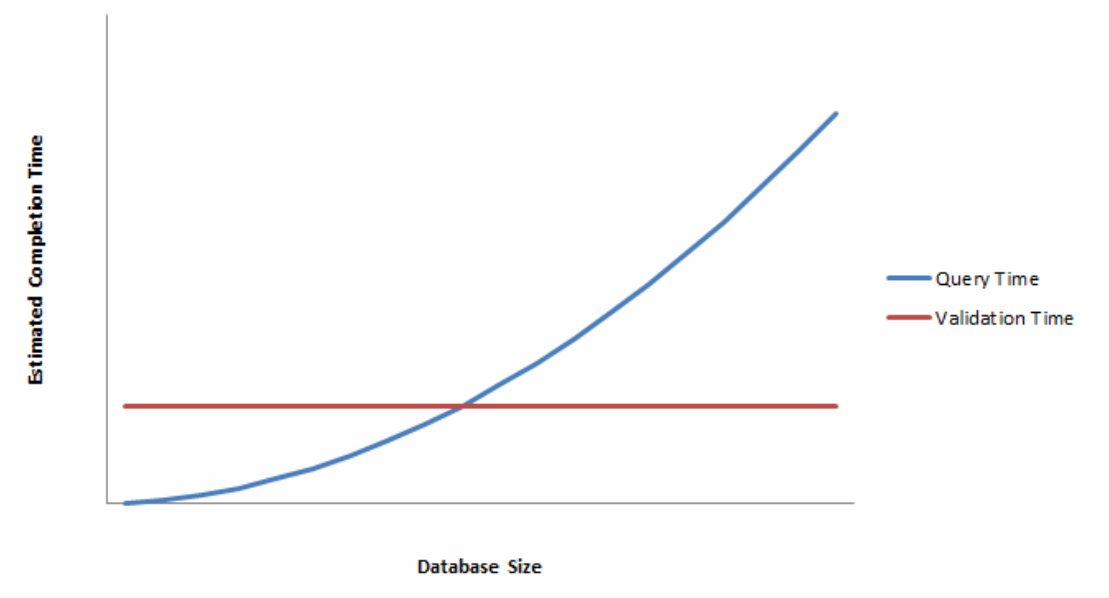
\includegraphics[scale=0.25]{expectation.png}
     \caption{An expected performance comparison of validating a single query and querying databases of various sizes.}
    \label{figure:expectation}
\end{figure}

In this paper, we discuss various methods for validating temporal queries, present our implementation of a temporal database with range queries, and describe an experiment to determine the time costs of adding a validation step to query plans.

\section{Temporal Queries over Streams}
The work by Li et al. introduces a new, interval-based query operator largely based on the temporal relation classifications described by Allen~\cite{Allen:1983}. The following classifications enumerate the various possible relations between intervals, with ts and te representing the start and end times of an event, respectively:

\begin{table}[!ht]\centering
\begin{tabular}{|c|c|}\hline
\textbf{Temporal Relation} & \textbf{Temporal Algebra}\\\hline
$e$ before $e'$ & $(e.te < e'.ts)$\\\hline
$e$ after $e'$ & $(e.ts > e'.te)$\\\hline
$e$ during $e'$ & $(e.ts > e'.ts) ^ (e.te < e'.te)$ \\\hline
$e$ contain $e'$ & $(e.ts < e'.ts) ^ (e.te > e'.te)$ \\\hline
$e$ meets $e'$ & $(e.te = e'.ts)$ \\\hline
$e$ met by $e'$ & $(e.ts = e'.te)$ \\\hline
$e$ overlap $e'$ & $(e.ts < e'.ts) ^ (e.te > e'.ts) ^ (e.te < e'.te)$ \\\hline
$e$ overlapped by $e'$ & $(e.ts > e'.ts) ^ (e.ts < e'.te) ^ (e.te > e'.te)$ \\\hline
$e$ start $e'$ & $(e.ts = e'.ts) ^ (e.te < e'.te)$ \\\hline
$e$ started by $e'$ & $(e.ts = e'.ts) ^ (e.te > e'.te)$ \\\hline
$e$ finish $e'$ & $(e.ts > e'.ts) ^ (e.te = e'.te)$ \\\hline
$e$ finished by $e'$ & $(e.ts < e'.ts) ^ (e.te = e'.te)$ \\\hline
$e$ equal $e'$ & $(e.ts = e'.ts) ^ (e.te = e'.te)$ \\\hline
\end{tabular}
\caption{Allen's 13 temporal relations. $e$ is an event whose start time is $e.ts$ and end time is $e.te$.}\label{tab:relations}
\end{table}

Given this set of relations, Li et al define ISEQ, a query processor designed to look for sets of relations between intervals. This processor, however, makes the assumption that any query provided to it will be valid (that is to say, logically consistent). For example, a query searching for two intervals which occur before each other and after each other should be rejected by a validator before being sent to the query processor.

While validation of the query is not, strictly speaking, a complex endeavor in terms of algorithm design, it can still be computationally costly depending on the query itself. This parallels a similar concern in query optimization. If a query optimization would take longer than actually running the query on the database, then doing so provides no real benefit. This is shown by Ilyas et al~\cite{Ilyas:2003}, who explore some methods for meta-optimization (i.e. selecting an appropriate level of optimization) in order to balance the cost of optimization with the query cost.
Of course, a validation process is not really capable of adjusting its resolution in the same way a meta-optimizer might. Partially validating a query would likely provide few gains as the true goal is to throw out bad queries without having to access the database at all. This can only be done if a query is entirely validated and deemed either consistent, at which point it is processed by ISEQ, or deemed inconsistent and rejected.

\section{Validation of Temporal Logic}
The actual cost of validation depends on two factors: the query length and the validation method.  Generally speaking, the validation of a temporal based query is a difficult problem.  When formally represented, a query of this type leads to a conjunction of relational clauses.  These clauses, each representing the relationship between to points in time, must all be concurrently satisfiable in order for the possibility of the query returning a set of satisfying records.  This is simply another case of the Boolean Satisfiability Problem (SAT), a problem which has been proven to be NP-hard ~\cite{Cook:1971}.

Allen's Temporal Relationships~\cite{Franke:2011} is an implementation of Allen's 13 relations shown in~\ref{tab:relations}. The library includes path consistency validation as proposed by Allen. Due to the limited number of existing validators for Allen's Temporal Logic (ATL), however, it may be more beneficial to convert queries into a more widely used formalism. Though converting the queries is not free, the savings of using a highly optimized, existing validator may outweigh these costs. Rosu and Bensalem~\cite{Rosu:2006} describe a linear translation from ATL to Linear Temporal Logic (LTL), allowing LTL validation techniques to be used on relations expressed in ATL.
For example, by converting the queries to LTL, it may be possible for AI planning techniques such as TLPlan~\cite{Bacchus:1998} to be used. This method would essentially treat the temporal relationships as a partially ordered set of constraints. Then, rather than using an existing validator, ATL can be simplified to a directed graph representation, where an edge between two time points (a, b) represents a dependency, namely that a must precede b. Inconsistencies can then be detected by looking for cycles in the graph with a topological sort~\cite{Pearce:2004} and, if found, the query is considered invalid.  The benefit of this approach is that its complexity is $O(V + E)$ where $V$ is the number of vertices in the graph and $E$ is the number of edges.  This is at worst $O(N!)$, but is considerably less in the average case.

Unfortunately, this method will only work under a restricted set of interval relationships. It does not, for example, cover the relationships in which two event times must be equal.  At best, we can approximate this by merging the vertices that represent the two values in the graph, taking the conjunction of their edges to be the edges of the new vertex.  In this way we assure that each value is constrained by the same temporal dependencies, but this still does not ensure that the values are actual equal.

Additionally, this approach does not generalize well as it can not handle disjunctive operators (e.g., less than or equal to).  When adding a disjunctive operator to an existing dependency graph, one can simply clone the graph and then add one of constituent operators to each graph.  Thus, one graph will represent the case that the values are equal and the other graph represents when they are not.  While this works, it unfortunately destroys the gains we would get from using this dependency graph approach.  By creating clones for each disjunctive operator, a search tree has been generated in which each node is a graph representation of the query and each disjunctive operator creates a new branch in this tree.  This leads to an overall complexity of $O(V + E)^d$, where $d$ is the number of disjunctive operators in the query.  This is much worse than we could do by simply approaching the problem as a SAT problem.

Armando et al.~\cite{Armando:1999} describe SAT-based validation techniques specifically for temporal logic expressed in disjunctive normal form (DNF). As any logical formula can be converted to DNF, we can simply convert temporal queries and then run them through a SAT solver. If the DNF formula is satisfiable, then the original query is valid. This method has the advantage of allowing us to leverage the extensive work on the SAT problem without needlessly constraining our queries (as the solutions above do).  
\section{Implementation}
\subsection{Generating Interval Formulas}
In order to prevent any unintentional bias that may be introduced by hand-crafting queries, we have instead created an automated query generator.  This generator can produce any number of queries, of any size, and can ensure the satisfiability of the queries it generates.  Using this, we have generated a set of queries ranging across the various parameters necessary to test our full query procedure and to gather the needed data to either confirm or contradict our hypothesis.

This generator begins by instantiating the parameterized number of intervals.  For each interval a starting point and an end point is created.  The system then randomly selects from one of the thirteen different interval relationships as defined by Allen.  Finally, it selects two of the instantiated intervals and, using the mapping from interval relationships to endpoint relationships in Table ~\ref{tab:relations}, it adds a new clause to the query.  It will continue to do this until the requisite number of clauses have been created.  So, for example, a query might be generated looking for an interval that is ``finished by'' another.  This query would appear thusly:  \texttt{x[0] < x[2], x[1] == x[3]}.  Here, each interval is represented by its start and end points as the elements \texttt{x[$2i$]} and \texttt{x[$2i+1$]}, respectively (where $i$ is the interval number).  For simplicity, all intervals are represented in a single array named \texttt{x}.

Except for the fact that the clauses are generated from a particular domain (Allen's relationships), query construction has occurred under no real restrictions thus far.  While the intervals were created to fill the query they had no actual values.  At this point, the query generator determines whether or not the query is satisfiable.  In this way, we can control which type of query is being generated at any given time and can be selective in our testing.  While it may be less efficient to generate a query, test it for satisfiability, and repeat until a query that is appropriately satisfiable is generated, the complexity of implementing a system that can deterministically generate an appropriate query is so high that it is practically infeasible.  Granted, a naive approach to this problem could deterministically generate queries of a specific satisfiability, but the concern is the bias that this may introduce.  For example, a system could easily make any query unsatisfiable by adding the contradiction to the first clause, but this would mean all unsatisfiable queries are unsatisfiable in the same way, which may affect the overall time necessary to determine satisfiability.  This sort of bias needs to be avoided.

Determination of a query's satisfiability is done in the same way as it is done for actual runtime testing.  First, the domain across which the intervals exist is specified.  Given that our interest is in timestamps, the start and end points of each interval is defined to be in the real numbers.  Thus, $\forall i, i_{start}, i_{end} \in \mathbb{R}$, where $i$ is an interval.  Once this is done, a series of constraints is added to the query to ensure that the intervals are properly represented.  More specifically, it is also necessary that the start points of all intervals occur before the end points.  If we generate a query and determine that it is satisfiable without enforcing this, we may find that with real data this query isn't actually satisfiable at all.  Thus, for every interval $i$, the clause \texttt{x[$2i$] < x[$2i+1$]} is added.  In this way, we can be sure that when the generator produces what it considers to be a satisfiable query that it is in fact doing so. 

\subsection{Converting Formulas to SQL Queries}
To use the formula as a SQL query, the table needed to be joined with itself depending on the number of intervals in the formula. However, with a large amount of joins, it becomes very costly to generate and store all results in memory. Thus, for experimentation purposes, we only return the \textit{count} of the results fulfilling the formula (e.g., \texttt{SELECT count(*) ...}). In the formula representation of interval logic, even-numbered indices represent interval start times and odd-numbered indices are finish times. Then, all variables of the form x[$2n$] are translated as \texttt{x$n$.start} and variables of the form x[$2n+1$] are translated as \texttt{x$n$.finish}. These transformations are set as the \texttt{WHERE} clause in the query.

For example, the input \texttt{x[0] < x[2], x[1] == x[3]} would be converted to the query \texttt{SELECT count(*) FROM medium x1, medium x2 WHERE x1.start < x2.start AND x1.finish = x2.finish}
\section{Experiment}
We conducted an experiment to study the performance effects of including a validation step in the query plan. 
\subsection{Experimental Design}
The experiment employed a 4x4x2 mixed factorial design. The three factors (and their treatments) were query length by number of intervals (2; 3; 4; and 6), database size by number of documents (1,000;  5,000; 25,000; and 50,000), and query satisfiability (satisfiable, unsatisfiable). The satisfiable queries were not run on the 50,000 item table or with queries of length 6 due of the exponential growth in time to run these queries.

The dataset used in the experiments were sampled from a total of 638,182 Twitter data items (tweets) collected between May 2, 2012 and June 10, 2012. Each entry contains the text of the tweet (``text''), the date-timestamp that the tweet was sent (``start''), and a ``finish''  date-timestamp which was fabricated by adding 1 second to the start time for every character in the tweet text. The entire dataset of 638,182 tweets was randomly sampled with a uniform distribution to create smaller databases of size 1,000, 10,000, 25,000 and 50,000 tweets to create the small and medium databases, respectively. The large database consists of the entire Twitter dataset. 

\subsection{Experimental Setup}
This project combines several pieces of off-the-shelf software in order to build a complete query system. Below is a list of this software and a brief justification of their selection:

\textbf{Server:} All experiments were performed on a KVM virtual machine running Gentoo Linux with one 3GHz CPU and 8GiB of RAM. 

\textbf{Database System:} The database server was Percona Server~\cite{Percona:2013}, a fork of MySQL~\cite{Oracle:2013},  a free, open source, relational database management system. The tables were loaded as \texttt{MEMORY} tables because they were small enough to fit into memory and this decreased speed to query. For indexes, B-Trees were created and used in place of the default Hash indices because they are more efficient for range and inequality queries.\cite{SQL:btree}

\textbf{SAT Solver:} Boolean satisfiability will be determined by Z3~\cite{DeMoura:2008}, a boolean satisfaction and optimization problem solver developed and maintained by Microsoft Research. This state of the art library is flexible, full featured, and robust and will allow us to concentrate on our experimentation rather than on implementing the necessary tools.  Additionally, it comes with an easy to use Python API.

\textbf{Project Management:} For project management and software version control, we use a private repository on GitHub~\cite{GitHub:2013}, a web-based hosting service which uses the Git versioning system. Github also offers a bug tracking system and a corresponding wiki which will allow for smoother collaboration.

\textbf{Language:} The temporal logic and validator was implemented in Python, which was chosen for its familiarity to the developers and because many packages exist for boolean logic validation.
\section{Results}
\subsection{Unsatisfiable Queries}
Timing results for the unsatisfiable queries are shown in Table~\ref{tab:unsat-results}. 

\begin{table*}
\begin{tabular}{|c||c||c|c|c|c|}\hline
\multirow{2}{*}{Query Length (intervals)} & \multirow{2}{*}{Validation Time (seconds)} &  \multicolumn{4}{|c|}{Query Time (seconds)} \\\cline{3-6}
 & & 1,000 & 10,000 & 25,000 & 50,000  \\\hline\hline
2 & 0.003340 & 0.000403 & 0.000812 & 0.002631 & 0.005768 \\\hline
3 & 0.003615 & 0.000406 & 0.000851 & 0.002636 & 0.005755\\\hline
4 & 0.004189 & 0.000943 & 0.011535 & 0.035187 & 0.029022\\\hline
6 & 0.005631 & 0.000942 & 0.001406 & 0.007416 & 0.006392 \\\hline
\end{tabular}
\caption{Timing results (in seconds) of validating and running unsatisfiable queries.}\label{tab:unsat-results}
\end{table*}

Overall, both validating and running unsatisfiable queries were extremely quick, with times under 0.01 seconds in most cases. Graphs of the results for each query length are shown in Figure~\ref{fig:unsat-graphs}.

\begin{figure}
\begin{subfigure}[b]{0.45\textwidth}
\centering
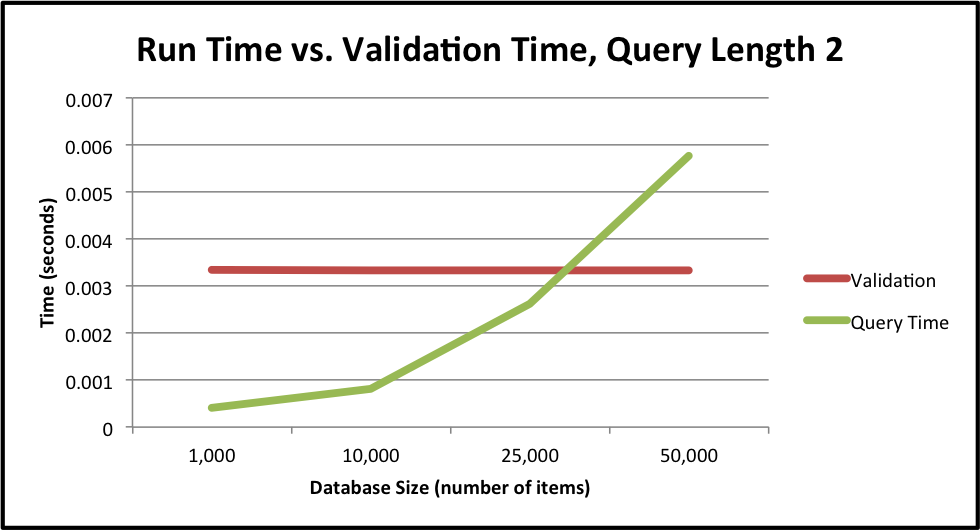
\includegraphics[width=\textwidth]{charts/unsat_2_graph}
\caption{Query Length 2}
\label{fig:unsat2}
\end{subfigure}%
\quad
\begin{subfigure}[b]{0.45\textwidth}
\centering
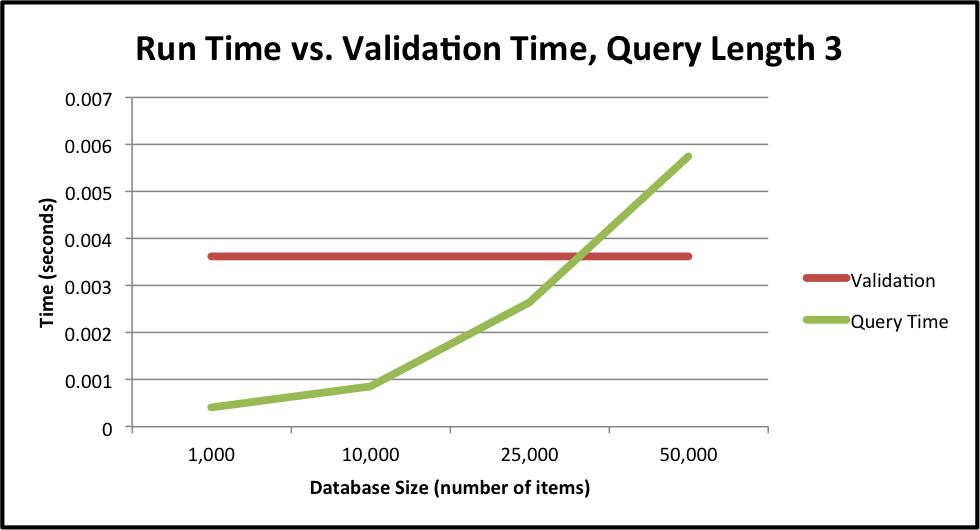
\includegraphics[width=\textwidth]{charts/unsat_3_graph}
\caption{Query Length 3}
\label{fig:unsat3}
\end{subfigure}
\quad
\begin{subfigure}[b]{0.45\textwidth}
\centering
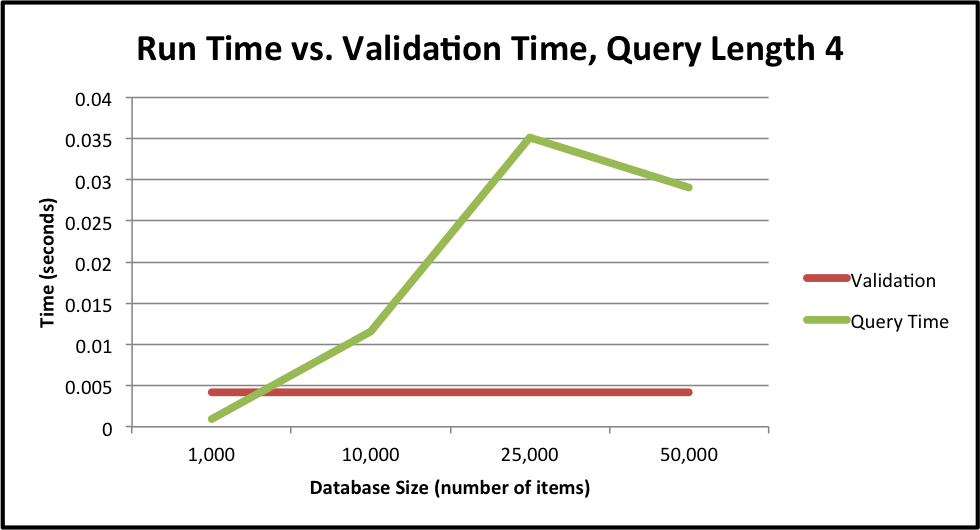
\includegraphics[width=\textwidth]{charts/unsat_4_graph}
\caption{Query Length 4}
\label{fig:unsat4}
\end{subfigure}
\quad
\begin{subfigure}[b]{0.45\textwidth}
\centering
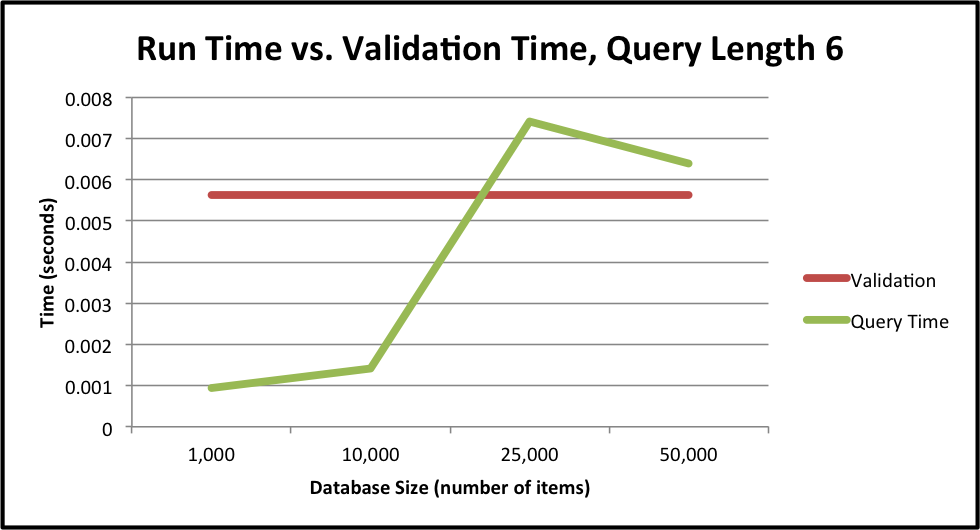
\includegraphics[width=\textwidth]{charts/unsat_6_graph}
\caption{Query Length 6}
\label{fig:unsat6}
\end{subfigure}

\caption{Graphs of validation and query time results (in seconds) for each query length versus database size.}\label{fig:unsat-graphs}
\end{figure}
\subsection{Satisfiable Queries}
Timing results for the unsatisfiable queries are shown in Table~\ref{tab:sat-results}. 

\begin{table*}
\begin{tabular}{|c||c||c|c|c|}\hline
\multirow{2}{*}{Query Length (intervals)} & \multirow{2}{*}{Validation Time (seconds)} &  \multicolumn{3}{|c|}{Query Time (seconds)} \\\cline{3-5}
 & & 1,000 & 10,000 & 25,000  \\\hline\hline
2 & 0.002887 & 0.029402 & 2.930172 & 16.173374 \\\hline
3 & 0.00384 & 0.182679 & 767.943567 & 5777.629936 \\\hline
4 & 0.004405 & 0.001026 & 71.94892 & 641.795355 \\\hline
\end{tabular}
\caption{Timing results (in seconds) of validating and running satisfiable queries.}\label{tab:sat-results}
\end{table*}

\subsubsection{Validation and Query Times versus Database Size per Query Length} 
Overall, both validating and running unsatisfiable queries were extremely quick, with times under 0.01 seconds in most cases. Graphs of the results for each query length are shown in Figure~\ref{fig:sat-graphs}.

\begin{figure}
\begin{subfigure}[b]{0.45\textwidth}
\centering
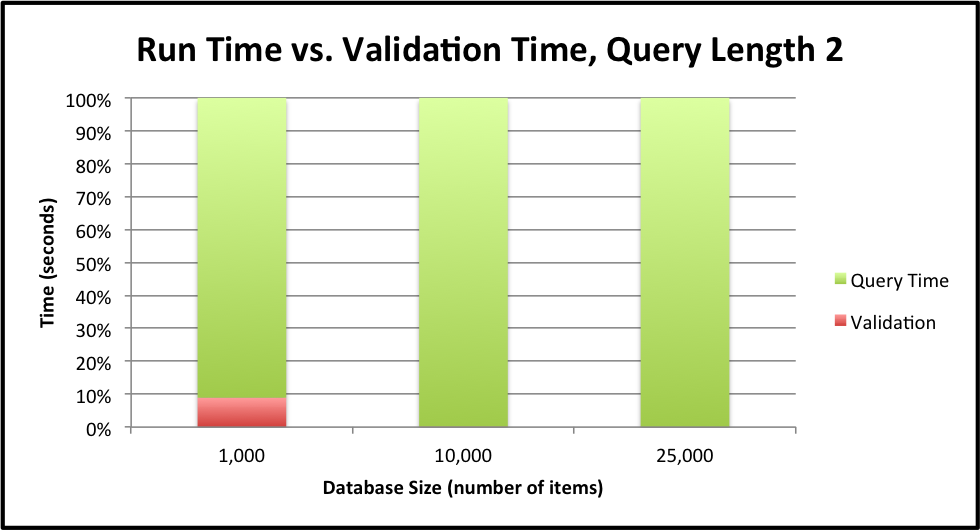
\includegraphics[width=\textwidth]{charts/sat_2_graph}
\caption{Query Length 2}
\label{fig:sat2}
\end{subfigure}%
\quad
\begin{subfigure}[b]{0.45\textwidth}
\centering
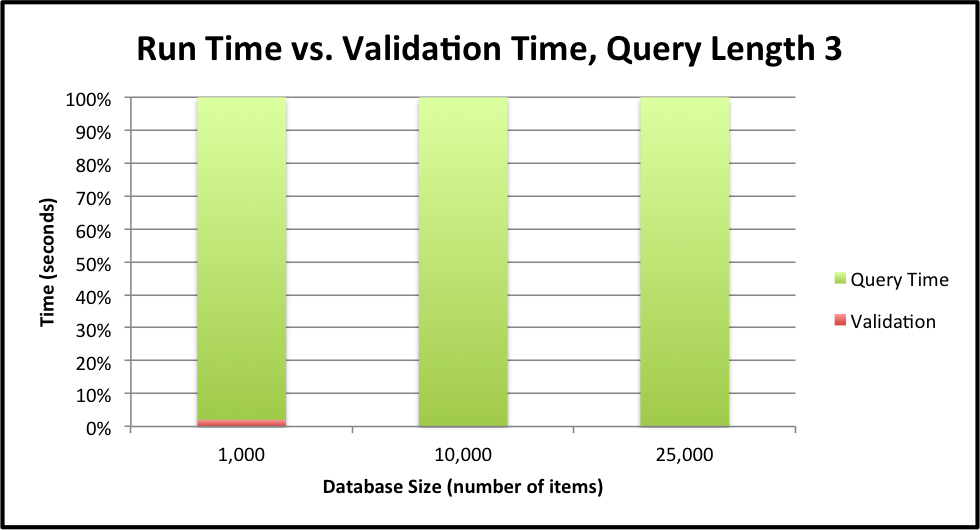
\includegraphics[width=\textwidth]{charts/sat_3_graph}
\caption{Query Length 3}
\label{fig:sat3}
\end{subfigure}
\quad
\begin{subfigure}[b]{0.45\textwidth}
\centering
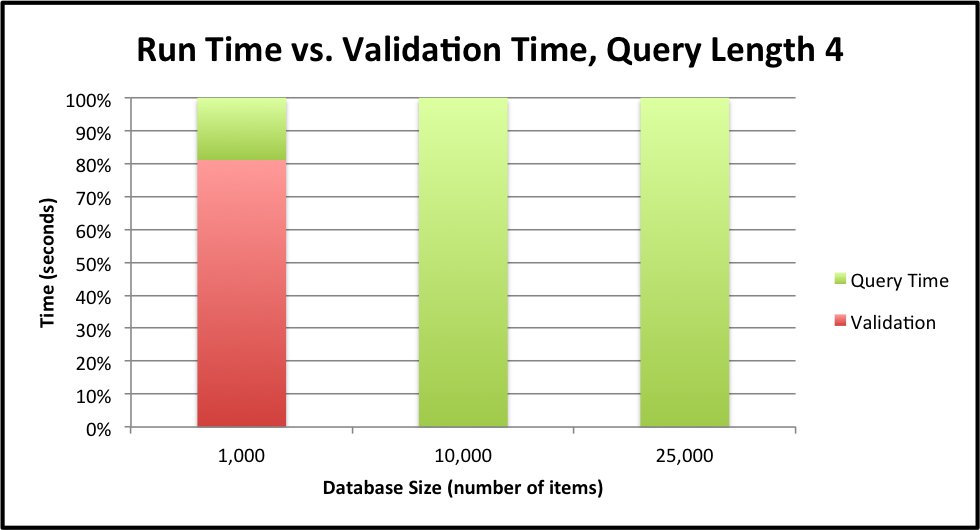
\includegraphics[width=\textwidth]{charts/sat_4_graph}
\caption{Query Length 4}
\label{fig:sat4}
\end{subfigure}

\caption{Graphs of validation and query time results (in seconds) for each query length versus database size.}\label{fig:sat-graphs}
\end{figure}

\section{Conclusions and Future Work}
Our original prediction is supported by the results of the unsatisfiable query running times. In all cases, there was a point where validating an unsatisfiable query was more efficient than running it. For query lengths 2 and 3, this point was between 25,000 and 50,000 items, for length 4 it was between 1,000 and 10,000 items, and for length 6, querying became more inefficient with between  10,000 and 25,000 items.

It appears that longer queries (length 4 and 6) combined with a larger database (50,000 items) runs more efficiently than the same query on smaller databases (25,000 items or less). 

This additional is justified in the satisfiable query step as well, because all validations times are a very small percentage of the query run time, meaning negligible performance effects of running the validator, as per Amdahl's Law.\cite{amdahl:1967} The exception is query length 4 on a small database, which takes up to 80\% of the run time, but the actual values of the runtimes are so small (0.0028s) that this is still a very small impact on runtime. 

Due to time and system constraints, there are many limitations to our experiment. Firstly, we only ran a single query of each class and length combination. In future evaluations, a more diverse set of queries may provide more accurate real-world behavior. Additionally, each query was only timed for one run, whereas it would be more accurate to average multiple iterations of the same query. Lastly, due to limited system resources, our database sizes and query lengths were quite small and short. A more realistic and beneficial evaluation would need to be done on larger database sizes with queries involving more intervals.

\bibliographystyle{plain}
\bibliography{intervals}
\end{document}